\documentclass{standalone}
\usepackage{tikz}
\usetikzlibrary{patterns, positioning}
\usepackage[sfdefault]{ClearSans} %% option 'sfdefault' activates Clear Sans as the default text font
\usepackage[T1]{fontenc}

\begin{document}
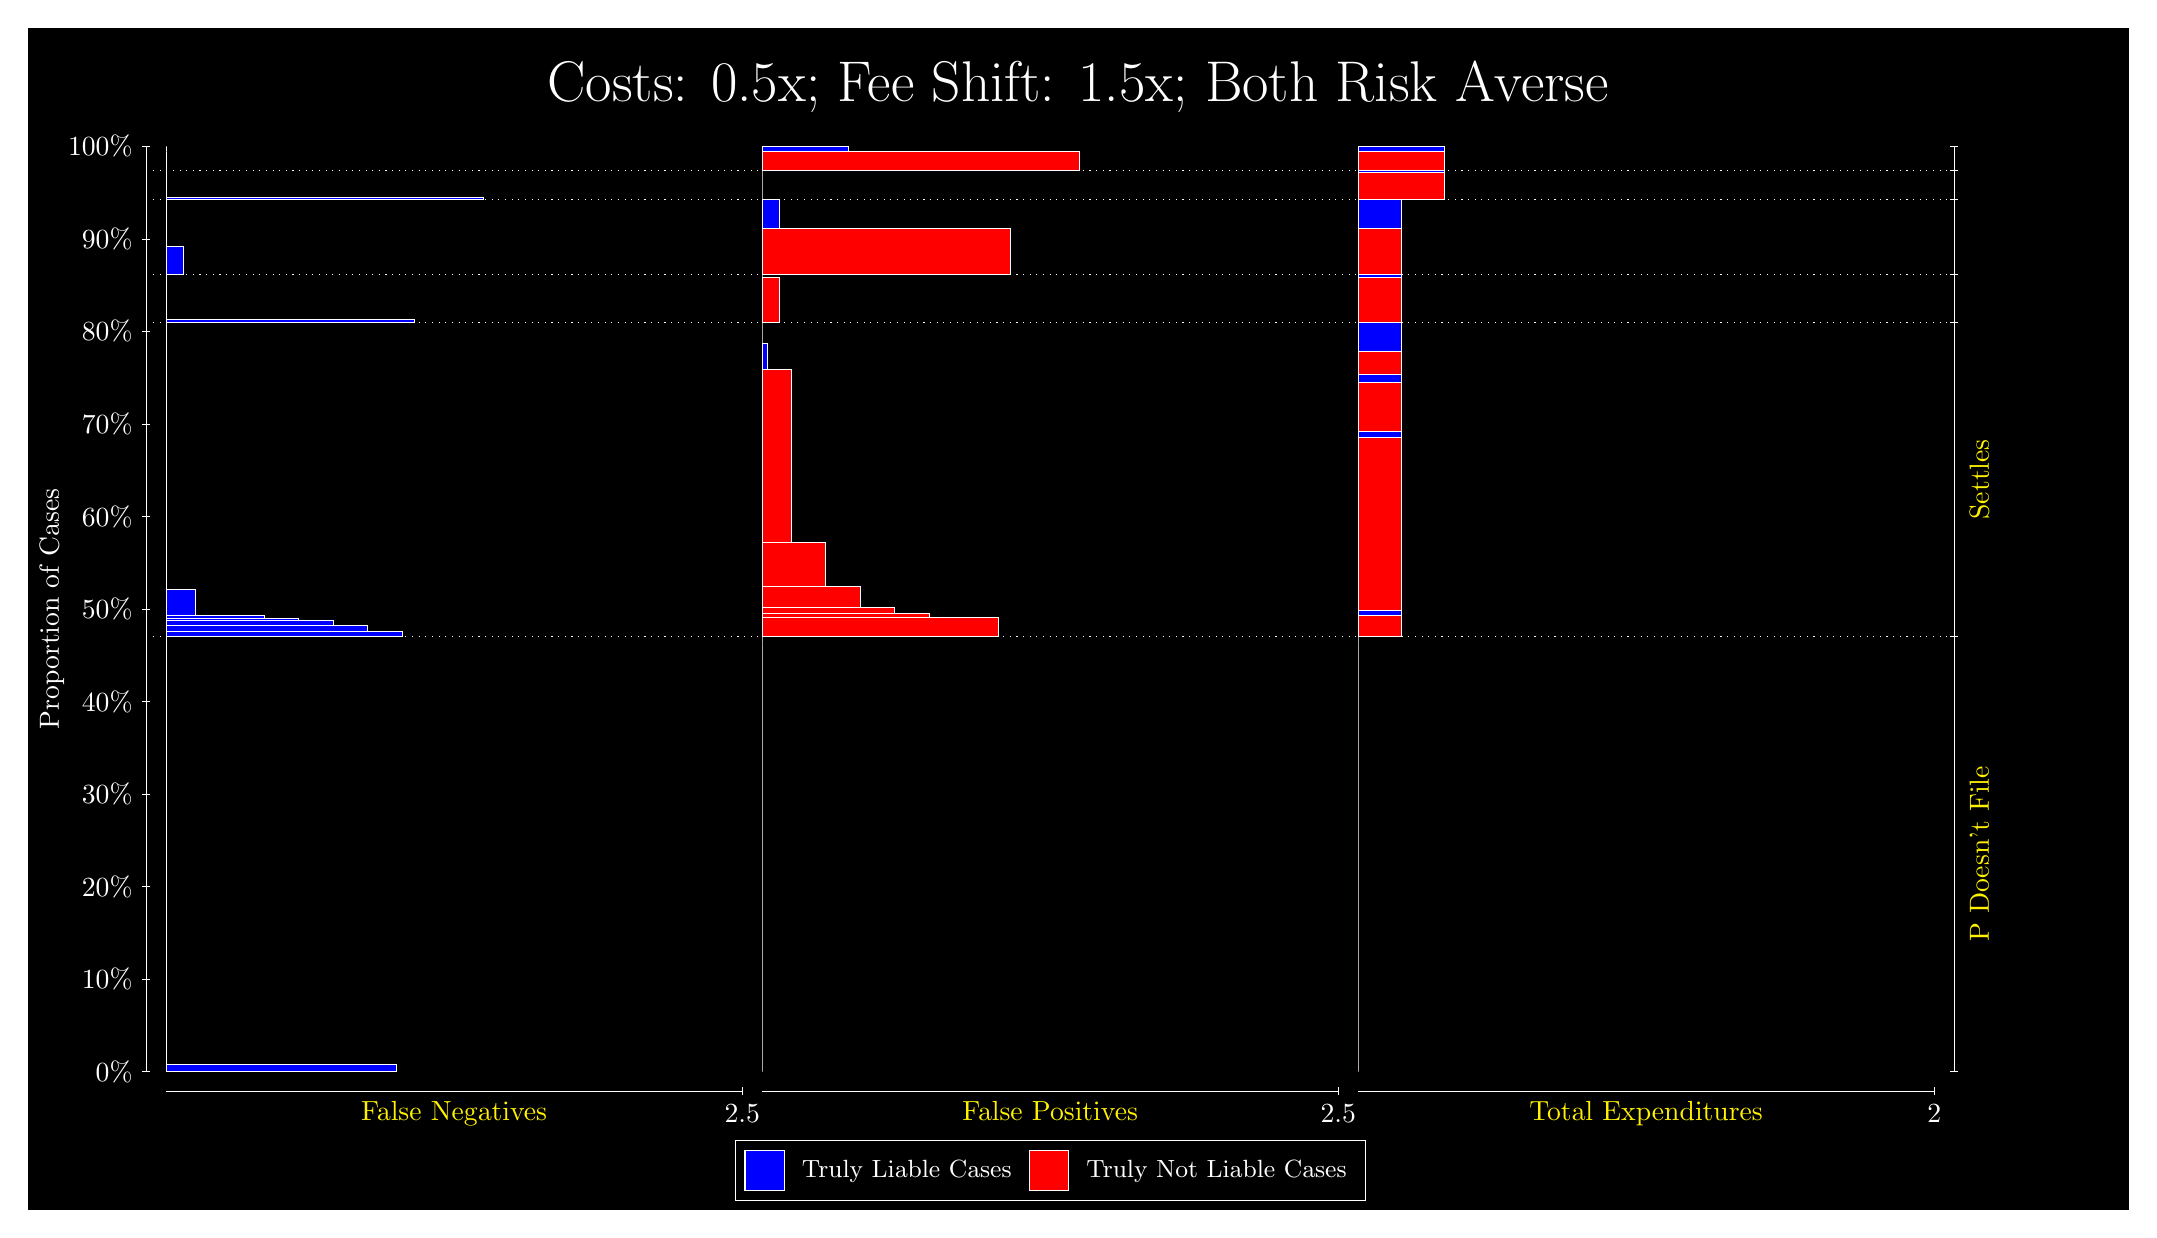
\begin{tikzpicture}
\draw[fill=black] (0,0) rectangle (26.667,15);
\draw[text=white] (0,13.5) rectangle (26.667,15) node[midway] {\huge Costs: 0.5x; Fee Shift: 1.5x; Both Risk Averse};
\draw[white, very thin] (1.5,1.75) -- (1.5,13.5);
\node[rotate=90, text=white, anchor=center] at (0.3, 7.625) {Proportion of Cases};
\draw[white, very thin] (1.45,1.75) -- (1.55,1.75);
\node[text=white, anchor=east] at (1.45, 1.75) {0\%};
\draw[white, very thin] (1.45,2.925) -- (1.55,2.925);
\node[text=white, anchor=east] at (1.45, 2.925) {10\%};
\draw[white, very thin] (1.45,4.1) -- (1.55,4.1);
\node[text=white, anchor=east] at (1.45, 4.1) {20\%};
\draw[white, very thin] (1.45,5.275) -- (1.55,5.275);
\node[text=white, anchor=east] at (1.45, 5.275) {30\%};
\draw[white, very thin] (1.45,6.45) -- (1.55,6.45);
\node[text=white, anchor=east] at (1.45, 6.45) {40\%};
\draw[white, very thin] (1.45,7.625) -- (1.55,7.625);
\node[text=white, anchor=east] at (1.45, 7.625) {50\%};
\draw[white, very thin] (1.45,8.8) -- (1.55,8.8);
\node[text=white, anchor=east] at (1.45, 8.8) {60\%};
\draw[white, very thin] (1.45,9.975) -- (1.55,9.975);
\node[text=white, anchor=east] at (1.45, 9.975) {70\%};
\draw[white, very thin] (1.45,11.15) -- (1.55,11.15);
\node[text=white, anchor=east] at (1.45, 11.15) {80\%};
\draw[white, very thin] (1.45,12.325) -- (1.55,12.325);
\node[text=white, anchor=east] at (1.45, 12.325) {90\%};
\draw[white, very thin] (1.45,13.5) -- (1.55,13.5);
\node[text=white, anchor=east] at (1.45, 13.5) {100\%};

\draw[white, very thin] (24.457,1.75) -- (24.457,13.5);
\draw[white, very thin] (24.407,1.75) -- (24.507,1.75);
\node[anchor=west] at (24.407, 1.75) {};
\draw[white, very thin] (24.407,7.2757) -- (24.507,7.2757);
\node[anchor=west] at (24.407, 7.2757) {};
\draw[white, very thin] (24.407,11.265) -- (24.507,11.265);
\node[anchor=west] at (24.407, 11.265) {};
\draw[white, very thin] (24.407,11.869) -- (24.507,11.869);
\node[anchor=west] at (24.407, 11.869) {};
\draw[white, very thin] (24.407,12.822) -- (24.507,12.822);
\node[anchor=west] at (24.407, 12.822) {};
\draw[white, very thin] (24.407,13.198) -- (24.507,13.198);
\node[anchor=west] at (24.407, 13.198) {};
\draw[white, very thin] (24.407,13.5) -- (24.507,13.5);
\node[anchor=west] at (24.407, 13.5) {};

\draw[white, very thin, fill=blue] (1.75,1.75) rectangle (4.6775,1.8393);
\draw[white, very thin, fill=red] (1.75,1.8393) rectangle (1.75,7.2757);
\draw[white, very thin, fill=blue] (1.75,7.2757) rectangle (4.7507,7.3451);
\draw[white, very thin, fill=blue] (1.75,7.3451) rectangle (4.3116,7.4166);
\draw[white, very thin, fill=blue] (1.75,7.4166) rectangle (3.8725,7.4817);
\draw[white, very thin, fill=blue] (1.75,7.4817) rectangle (3.4333,7.5087);
\draw[white, very thin, fill=blue] (1.75,7.5087) rectangle (2.9942,7.5443);
\draw[white, very thin, fill=blue] (1.75,7.5443) rectangle (2.1159,7.8748);
\draw[white, very thin, fill=red] (1.75,7.8748) rectangle (1.75,11.265);
\draw[white, very thin, fill=blue] (1.75,11.265) rectangle (4.8971,11.302);
\draw[white, very thin, fill=red] (1.75,11.302) rectangle (1.75,11.869);
\draw[white, very thin, fill=blue] (1.75,11.869) rectangle (1.9696,12.227);
\draw[white, very thin, fill=red] (1.75,12.227) rectangle (1.75,12.822);
\draw[white, very thin, fill=blue] (1.75,12.822) rectangle (5.7754,12.848);
\draw[white, very thin, fill=red] (1.75,12.848) rectangle (1.75,13.198);
\draw[white, very thin, fill=red] (1.75,13.198) rectangle (1.75,13.435);
\draw[white, very thin, fill=blue] (1.75,13.435) rectangle (1.75,13.5);
\draw[white, very thin, fill=red] (9.3189,1.75) rectangle (9.3189,7.1864);
\draw[white, very thin, fill=blue] (9.3189,7.1864) rectangle (9.3189,7.2757);
\draw[white, very thin, fill=red] (9.3189,7.2757) rectangle (12.32,7.5133);
\draw[white, very thin, fill=red] (9.3189,7.5133) rectangle (11.441,7.5701);
\draw[white, very thin, fill=red] (9.3189,7.5701) rectangle (11.002,7.6435);
\draw[white, very thin, fill=red] (9.3189,7.6435) rectangle (10.563,7.9152);
\draw[white, very thin, fill=red] (9.3189,7.9152) rectangle (10.124,8.4676);
\draw[white, very thin, fill=red] (9.3189,8.4676) rectangle (9.6848,10.666);
\draw[white, very thin, fill=blue] (9.3189,10.666) rectangle (9.3921,10.997);
\draw[white, very thin, fill=blue] (9.3189,10.997) rectangle (9.3189,11.265);
\draw[white, very thin, fill=red] (9.3189,11.265) rectangle (9.5384,11.832);
\draw[white, very thin, fill=blue] (9.3189,11.832) rectangle (9.3189,11.869);
\draw[white, very thin, fill=red] (9.3189,11.869) rectangle (12.466,12.463);
\draw[white, very thin, fill=blue] (9.3189,12.463) rectangle (9.5384,12.822);
\draw[white, very thin, fill=red] (9.3189,12.822) rectangle (9.3189,13.172);
\draw[white, very thin, fill=blue] (9.3189,13.172) rectangle (9.3189,13.198);
\draw[white, very thin, fill=red] (9.3189,13.198) rectangle (13.344,13.435);
\draw[white, very thin, fill=blue] (9.3189,13.435) rectangle (10.417,13.5);
\draw[white, very thin, fill=red] (16.888,1.75) rectangle (16.888,7.1864);
\draw[white, very thin, fill=blue] (16.888,7.1864) rectangle (16.888,7.2757);
\draw[white, very thin, fill=red] (16.888,7.2757) rectangle (17.437,7.5474);
\draw[white, very thin, fill=blue] (16.888,7.5474) rectangle (17.437,7.6126);
\draw[white, very thin, fill=red] (16.888,7.6126) rectangle (17.437,9.8112);
\draw[white, very thin, fill=blue] (16.888,9.8112) rectangle (17.437,9.8806);
\draw[white, very thin, fill=red] (16.888,9.8806) rectangle (17.437,10.506);
\draw[white, very thin, fill=blue] (16.888,10.506) rectangle (17.437,10.605);
\draw[white, very thin, fill=red] (16.888,10.605) rectangle (17.437,10.899);
\draw[white, very thin, fill=blue] (16.888,10.899) rectangle (17.437,11.265);
\draw[white, very thin, fill=red] (16.888,11.265) rectangle (17.437,11.832);
\draw[white, very thin, fill=blue] (16.888,11.832) rectangle (17.437,11.869);
\draw[white, very thin, fill=red] (16.888,11.869) rectangle (17.437,12.463);
\draw[white, very thin, fill=blue] (16.888,12.463) rectangle (17.437,12.822);
\draw[white, very thin, fill=red] (16.888,12.822) rectangle (17.986,13.172);
\draw[white, very thin, fill=blue] (16.888,13.172) rectangle (17.986,13.198);
\draw[white, very thin, fill=red] (16.888,13.198) rectangle (17.986,13.435);
\draw[white, very thin, fill=blue] (16.888,13.435) rectangle (17.986,13.5);
\draw[white, dotted] (1.5,7.2757) -- (24.457,7.2757);
\draw[white, dotted] (1.5,11.265) -- (24.457,11.265);
\draw[white, dotted] (1.5,11.869) -- (24.457,11.869);
\draw[white, dotted] (1.5,12.822) -- (24.457,12.822);
\draw[white, dotted] (1.5,13.198) -- (24.457,13.198);
\draw[white, very thin] (1.75,1.5) -- (9.0689,1.5);
\node[text=yellow, anchor=north] at (5.4094, 1.5) {False Negatives};
\draw[white, very thin] (9.0689,1.45) -- (9.0689,1.55);
\node[text=white, anchor=north] at (9.0689, 1.45) {2.5};

\draw[white, very thin] (9.3189,1.5) -- (16.638,1.5);
\node[text=yellow, anchor=north] at (12.978, 1.5) {False Positives};
\draw[white, very thin] (16.638,1.45) -- (16.638,1.55);
\node[text=white, anchor=north] at (16.638, 1.45) {2.5};

\draw[white, very thin] (16.888,1.5) -- (24.207,1.5);
\node[text=yellow, anchor=north] at (20.547, 1.5) {Total Expenditures};
\draw[white, very thin] (24.207,1.45) -- (24.207,1.55);
\node[text=white, anchor=north] at (24.207, 1.45) {2};

\node[text=yellow, centered, rotate=90] at (24.777, 4.5128) {P Doesn't File};
\node[text=yellow, centered, rotate=90] at (24.777, 9.2705) {Settles};





\draw (12.978300999999998,1.5) node[draw=none] (baseCoordinate) {};
\begin{scope}[align=center]
        \matrix[scale=0.5, draw=white, below=0.5cm of baseCoordinate, nodes={draw}, column sep=0.1cm]{
            \node[rectangle, draw, minimum width=0.5cm, minimum height=0.5cm, fill=blue] {}; &
            \node[draw=none, font=\small, text=white] (B) {Truly Liable Cases}; &
            \node[rectangle, draw, minimum width=0.5cm, minimum height=0.5cm, fill=red] {}; &
            \node[draw=none, font=\small, text=white] (B) {Truly Not Liable Cases}; \\
            };
\end{scope}

\end{tikzpicture}
\end{document}